% Draft manuscript for The Visual Computer (Springer).
% Before submission, port to the current Springer Nature LaTeX template (sn-jnl.cls) and follow
% the journal's author guidelines. Everything marked \todo{} must be completed or removed.
\documentclass[11pt]{article}
\usepackage[margin=2.5cm]{geometry}
\usepackage{amsmath,amssymb,amsthm}
\usepackage{graphicx}
\usepackage{booktabs}
\usepackage{xcolor}
\usepackage{algorithm}
\usepackage{algpseudocode}
\usepackage[hidelinks]{hyperref}
\usepackage[numbers,sort&compress]{natbib}

\newcommand{\todo}[1]{\textcolor{red}{[TODO: #1]}}
\newtheorem{proposition}{Proposition}
\graphicspath{{figures/}}

\title{From Photograph to Loom: Structure-Constrained Generation and Digitisation of Manipuri Textile Patterns}
\author{\todo{Author names and affiliations}}
\date{}

\begin{document}
\maketitle

\begin{abstract}
Handloom textiles of Manipur, such as the striped \emph{phanek} and the \emph{Moirang phee} with its
rows of temple-like motifs, are a living cultural heritage that has received little attention
from visual computing. We present a complete pipeline that (i) digitises photographs of textiles
into clean grids of \emph{design cells}, (ii) generates new designs with a masked discrete
diffusion transformer that operates directly on these weavable grids, and (iii) compiles any design
into loom-ready weaving instructions. The generator separates structure from colour through a
canonical palette representation and enforces mirror symmetry, repeats and stripes \emph{exactly}
by pooling predictions over symmetry orbits during sampling. The compiler produces
supplementary-weft drafts on single-colour, striped or plaid grounds, bounds float lengths with
staggered tie-downs, and exports standard WIF files, pick-up instructions, charts, yarn estimates
and a yarn-level fabric simulation. We contribute a consent-based dataset of digitised Manipuri
textiles \todo{size}, an evaluation protocol with palette-independent pattern statistics and
weavability metrics, and a study with Manipuri weavers \todo{summary of results}.
\end{abstract}

\noindent\textbf{Keywords:} cultural heritage; generative models; discrete diffusion; weaving;
textile design; digitisation

%==========================================================================================
\section{Introduction}

Manipur's handloom tradition is central to everyday and ceremonial life \todo{cite ethnographic /
government sources}. The \emph{phanek}, a wrap-around garment, is woven with characteristic
stripe sequences; the \emph{Moirang phee} carries borders of stepped, temple-like motifs and is
reported to be a registered Geographical Indication of India \todo{verify and cite the GI
registry}. Weaving such designs requires translating a pattern into a \emph{draft}: which warp
ends are lifted for every pick, which yarn colour is used, and how long floats are bound. Today
this translation is done by hand and the designs themselves live mostly in the memory of weavers
and in physical pieces.

Modern generative models produce compelling images but are a poor fit for this setting: their
outputs are continuous-valued pixels without the discrete grid, small palette and exact
repetitions of a woven design, and they offer no path to the loom. We argue that the right
representation is the grid of \emph{design cells} a weaver actually works with, and build the full
loop around it (Fig.~\ref{fig:pipeline}).

\paragraph{Contributions.}
\begin{itemize}
  \item A \textbf{grid-native generator}: masked discrete diffusion over canonical design-cell grids
        with style, colour-budget and domain conditioning, and \textbf{exact} structural control by
        \emph{orbit pooling} (Sec.~\ref{sec:model}).
  \item A \textbf{design-to-loom compiler} for supplementary-weft brocade on single-colour, striped or
        plaid grounds, with plaid inference from optical-mixture colours, provably float-bounded
        tie-downs, WIF export and pick-up instructions (Sec.~\ref{sec:compiler}).
  \item A \textbf{digitisation} method for textile photographs with orbit-pooled structure
        regularisation, and a synthetic benchmark with exact ground truth (Sec.~\ref{sec:digitise}).
  \item A \textbf{dataset} of digitised Manipuri textiles collected with informed consent, an
        \textbf{evaluation protocol}, a \textbf{study with weavers} and a physical weaving case study
        (Sec.~\ref{sec:experiments}). \todo{finalise}
\end{itemize}

%==========================================================================================
\section{Related work}

\paragraph{Generative models for discrete data.}
Masked generative transformers \cite{chang2022maskgit} iteratively unmask tokens of a quantised
image representation \cite{esser2021taming}. Discrete and masked diffusion models
\cite{austin2021structured,sahoo2024simple,shi2024simplified} provide a likelihood-based view of the
same process; diffusion transformers \cite{peebles2023scalable} with classifier-free guidance
\cite{ho2022classifier} are the standard backbone for continuous diffusion
\cite{ho2020denoising,rombach2022high}. We adopt masked diffusion directly on design cells (no
learned tokenizer), use 2-D rotary embeddings \cite{su2024roformer}, and add exact structural
constraints at sampling time.

\paragraph{Computational textiles.}
Compilers for machine knitting \cite{mccann2016compiler,narayanan2018automatic} and inverse
knitting from images \cite{kaspar2019neural} connect visual designs to fabrication instructions;
yarn-level appearance and design tools \cite{zhao2011building,irawan2012specular,leaf2018interactive}
model the look of fabric. Weaving drafts are exchanged in the WIF format \cite{wif1997}.
\todo{add work on weave design tools, jacquard design, and generative models for traditional
textiles (e.g. batik, kente, songket, Indian handloom); verify each reference}

\paragraph{Pattern and texture synthesis.}
Non-parametric \cite{efros1999texture} and neural \cite{gatys2015texture} texture synthesis
reproduce stationary statistics but not the exact symmetries and repeats of woven borders.

\paragraph{Digital cultural heritage.}
\todo{documentation and digitisation of crafts, community-centred methods, ethics of generative
models for cultural artefacts}

%==========================================================================================
\section{Background: Manipuri textiles}
\todo{Concise, sourced description of the textiles in the dataset (phanek types, Moirang phee,
Leirum phee, ...), looms (loin loom, frame looms), and techniques (warp/weft stripes,
supplementary weft). Have this section checked by Manipuri textile experts.}

%==========================================================================================
\section{Representation}
\label{sec:representation}

A design is a grid $X \in \{0,\dots,K-1\}^{H\times W}$ of palette indices with palette
$P \in [0,255]^{K\times 3}$. Column $j$ corresponds to $e$ warp ends (\emph{ends per cell}); rows run
along the warp and are woven from the bottom row up. We renumber colours by decreasing frequency
(ties by first occurrence), so slot $0$ is the most frequent colour --- usually the ground. This
\emph{canonical} form makes the model palette-agnostic: it predicts colour slots, and colours are
assigned afterwards by frequency-rank transfer from palettes observed in real textiles.

%==========================================================================================
\section{Grid-native generation}
\label{sec:model}

\paragraph{Masked diffusion.}
At time $t\in[0,1]$ every cell is independently replaced by a \texttt{MASK} token with probability
$r(t)$, $r(0)=0$, $r(1)=1$. A denoiser $p_\theta(x_i \mid X_t, c)$ predicts the colour of masked cells
given conditions $c$ (style, number of colours, synthetic/real domain). We train with the cosine
schedule $r(t)=\sin(\pi t/2)$ and the mean cross-entropy over masked cells \cite{chang2022maskgit}.
With the linear schedule $r(t)=t$, the negative ELBO
\begin{equation}
\mathcal{L}(X) = \mathbb{E}_{t\sim U(0,1)}\Big[\tfrac{1}{t}\sum_{i:\,X_t^i=\texttt{MASK}} -\log p_\theta(x_i\mid X_t,c)\Big]
\end{equation}
upper-bounds $-\log p_\theta(X\mid c)$ \cite{sahoo2024simple,shi2024simplified}; we report it in
bits per cell on held-out data.

\paragraph{Architecture.}
Each cell (colour slot or \texttt{MASK}) is embedded; the embeddings of a $p\times p$ patch are
concatenated and linearly projected to one token, so sequences have $HW/p^2$ tokens while every
cell keeps its own output logits. A DiT-style transformer \cite{peebles2023scalable,vaswani2017attention}
with axial 2-D rotary position embeddings \cite{su2024roformer}, QK-normalisation and SwiGLU MLPs
is conditioned through adaLN-Zero on the sum of style, colour-count and domain embeddings; each
condition has a learned null entry used for classifier-free guidance \cite{ho2022classifier}.

\paragraph{Exact structural control by orbit pooling.}
A symmetry (left--right mirror, top--bottom mirror, $180^\circ$ rotation, horizontal or vertical
repeat with period $\pi$, row or column stripes) induces a partition of the cells into orbits
$\mathcal{O}$ whose members must share a colour (Fig.~\ref{fig:orbits}). Sampling runs the reverse
process on orbits: at every step the per-cell log-probabilities are pooled,
\begin{equation}
\log q_O(k) = \frac{1}{|O|}\sum_{i\in O}\log p_\theta(x_i = k\mid X_t,c) - \log Z_O,
\end{equation}
one colour is drawn per masked orbit, and going from time $t$ to $t'<t$ each masked orbit is
revealed as a unit with probability $(r(t)-r(t'))/r(t)$, the ancestral step of the masking process
\cite{sahoo2024simple,shi2024simplified} (Alg.~\ref{alg:sample}). We also implement MaskGIT's
ordering \cite{chang2022maskgit}, which reveals the most confident orbits first (with annealed
Gumbel noise). It is mode-seeking: for styles with sparse motifs on a large ground it often returns
plain ground (Sec.~\ref{sec:experiments}).

\begin{proposition}
Every grid produced by orbit-pooled sampling is constant on every orbit. With sum pooling, the
pooled distribution equals the conditional of the factorised per-step proposal
$\prod_i p_\theta(x_i\mid X_t,c)$ given that all cells of an orbit are equal.
\end{proposition}
\begin{proof}
Each orbit receives exactly one colour, written to all its members, and known (inpainted) cells fix
their orbit. For the second claim, $\Pr(x_i=k\ \forall i\in O)\propto\prod_{i\in O}p_i(k)$.
\end{proof}
Mean pooling tempers the product (power $1/|O|$), which avoids over-confidence because cells of an
orbit share most of their context. Inpainting fixes known cells; large canvases are produced by
outpainting overlapping windows.

\begin{algorithm}[t]
\caption{Orbit-pooled sampling}\label{alg:sample}
\begin{algorithmic}[1]
\State orbits $\mathcal{O}$ from the symmetry; mark orbits containing known cells as unmasked
\For{$s = 0,\dots,S-1$}
  \State $t \gets 1-\tfrac{s}{S}$, \ $t' \gets 1-\tfrac{s+1}{S}$
  \State $\ell \gets$ guided logits of $p_\theta(\cdot\mid X, c)$; mask colour slots $\ge$ budget
  \State pool log-probabilities over each orbit; sample a colour $k_O$ for every masked orbit
  \State reveal each masked orbit with probability $(r(t)-r(t'))/r(t)$ (all of them when $t'=0$)
\EndFor
\end{algorithmic}
\end{algorithm}

%==========================================================================================
\section{From design to loom}
\label{sec:compiler}

\paragraph{Draft.}
A draft is a lift plan $L\in\{0,1\}^{P\times E}$ ($L_{pe}=1$: end $e$ raised on pick $p$, warp
visible on the face), warp and weft colours, pick kinds and the design row of every pick. Threading
(one shaft per distinct column of $L$), tie-up and treadling are derived exactly, which also gives
the number of shafts a dobby loom would need.

\paragraph{Ground planning.}
The compiler decides which cells the ground cloth can show: a single ground colour; weft or warp
stripes (rows/columns that are $\ge 90\%$ one colour); or a plaid. For plaids, colours whose CIEDE2000
\cite{sharma2005ciede2000} distance to the linear-light mixture of two other colours is below a
threshold are treated as crossings, and the warp and weft colour sequences are recovered by voting.
The plan explaining most cells is selected.

\paragraph{Supplementary weft and tie-downs.}
Remaining cells are woven with a supplementary weft: after each ground pick, one pattern pick per
colour of the row (continuous weft, floating on the back when hidden) or one inlay pick carrying
several colours. A visible run of $L>F$ ends would float too far; tie-down ends are raised on an
absolute lattice $\{x\in(a,b-1):(x-\varphi)\bmod F=0\}$ whose phase $\varphi$ alternates by $F/2$
between pattern picks (brick stagger, Alg.~\ref{alg:tie}).

\begin{proposition}
For $F\ge 2$, Algorithm~\ref{alg:tie} leaves every visible float of length at most $F$ and never
raises the first or last end of a run.
\end{proposition}
\begin{proof}[Sketch]
Between consecutive lattice points there are $F-1$ ends; the first lattice point lies within $F$
ends of the run start and the last within $F$ ends of the run end. Gaps that still exceed $F$
(short runs whose lattice points coincide with run ends) are split at their midpoint, which is an
interior end because the gap is at least $F+1\ge 3$.
\end{proof}

\begin{algorithm}[t]
\caption{Tie-down placement for one pattern pick}\label{alg:tie}
\begin{algorithmic}[1]
\For{each visible run $[a,b)$ with $b-a>F$}
  \State $T \gets \{x : a < x < b-1,\ (x-\varphi) \bmod F = 0\}$
  \While{some gap between consecutive points of $\{a-1\}\cup T\cup\{b\}$ exceeds $F$}
    \State add the gap's midpoint to $T$
  \EndWhile
  \State drop an edge tie if the merged float is still $\le F$; raise the ends in $T$
\EndFor
\end{algorithmic}
\end{algorithm}

\paragraph{Row balancing and outputs.}
Rows without pattern picks receive extra ground picks so that every design row occupies the same
length of cloth. The compiler exports WIF \cite{wif1997}, run-length pick-up codes (\emph{lift} /
\emph{leave down} counts per pattern pick), printable charts and yarn quantities, and renders the face
with a yarn-level model: a continuous ground cloth with visible pattern floats spreading over the
ground picks of their row (Fig.~\ref{fig:pipeline}).

%==========================================================================================
\section{Digitising photographs}
\label{sec:digitise}

The cloth is rectified from four corners with a homography \cite{hartley2004multiple}. The cell
lattice is found from sub-pixel edge points: the yarn period is detected and suppressed, and the
coarsest lattice whose chance-corrected edge coverage is within 90\% of the best lattice is
selected; boundaries are refined by dynamic programming. Cell colours are interquartile means of
the cell centres in linear light, which ignore tie-down dots but return optical mixtures for plaid
crossings. Colours are clustered in CIELAB (k-means++ \cite{arthur2007kmeans}) with an automatic
count, a cluster-aware multiplicative lighting model and removal of boundary-mixture clusters;
labels are denoised with ICM on a Potts model \cite{besag1986statistical} and regularised by
pooling costs over stripe, repeat and mirror orbits detected with foreground-weighted scores.

%==========================================================================================
\section{Experiments}
\label{sec:experiments}

\paragraph{Data.}
Procedural pretraining data comes from a grammar of stepped motifs and band layouts
(Fig.~\ref{fig:styles}). The real dataset contains \todo{N pieces / M designs, categories,
collection protocol and consent, splits by piece}.

\paragraph{Metrics.}
Palette-independent pattern statistics: Jensen--Shannon divergence between distributions of
$k\times k$ colour \emph{partitions} ($k=2,3$), Wasserstein distance between run-length
distributions along rows and columns, total variation of colour counts; symmetry and repeat scores;
diversity and nearest-neighbour novelty (flip- and palette-invariant Hamming distance); likelihood
(bits/cell); weavability (tie-downs per 100 cells, longest floats, dobby shafts).

\paragraph{Results.} \todo{E1 fidelity vs grammar / retrieval / autoregressive / image-space
baselines; E2 orbit pooling vs projection; E3 data efficiency; E4 weavability; E5 weaver study;
E6 woven case study.}

\paragraph{Sampling order.} The bias of confidence ordering is visible even without context: for
a stub denoiser that gives every cell the motif colour with probability 0.2, ancestral sampling
produced 20.2\,\% motif cells, MaskGIT ordering 1.8\,\% without and 9.6\,\% with Gumbel noise of
scale 4.5 (8 samples of $32\times32$ cells, 16 steps). In a preliminary run (4\,M-parameter model, procedural data only,
$32\times32$ cells, 24 samples per style) MaskGIT ordering with unit Gumbel noise and 16 steps
returned a single-colour grid for 75\,\% of Moirang phee samples and 46\,\% of motif-tile samples,
whereas ancestral sampling returned none. Ancestral sampling with 32 steps and guidance $w=1$ came
within 0.01 of the best $3\times3$ pattern-JS and 0.02 of the best row run-length distance among
the settings tried, and is our default.
\todo{repeat with the final models (part of the ablations)}

\paragraph{Digitisation (synthetic benchmark).}
Table~\ref{tab:digitise} reports results on synthetic photographs (perspective, blur, uneven
lighting, sensor noise, JPEG) of $40\times48$-cell designs with exact ground truth.
\todo{add the real-photo subset with manually corrected ground truth}

\begin{table}[t]
\centering
\caption{Digitisation on synthetic photographs (6 seeds per style). Assisted: corners and cell
counts given (cell accuracy). Automatic: corners only (pixel accuracy, resolution independent).
Clean: noise-free pixel-art inputs. Produced by \texttt{scripts/benchmark\_digitise.py}.}
\label{tab:digitise}
\begin{tabular}{lcccc}
\toprule
style & assisted & automatic & clean, automatic & clean, assisted exact \\
\midrule
phanek mayek naibi & 1.000 & 0.965 & 1.000 & 100\% \\
Moirang phee       & 0.999 & 0.960 & 1.000 & 100\% \\
banded motif       & 0.946 & 0.962 & 1.000 & 100\% \\
check              & 1.000 & 0.873 & 0.990 & 100\% \\
motif tile         & 0.994 & 0.957 & 0.987 & 100\% \\
\midrule
all                & 0.988 & 0.943 & 0.995 & 100\% \\
\bottomrule
\end{tabular}
\end{table}

\begin{figure}[t]
\centering
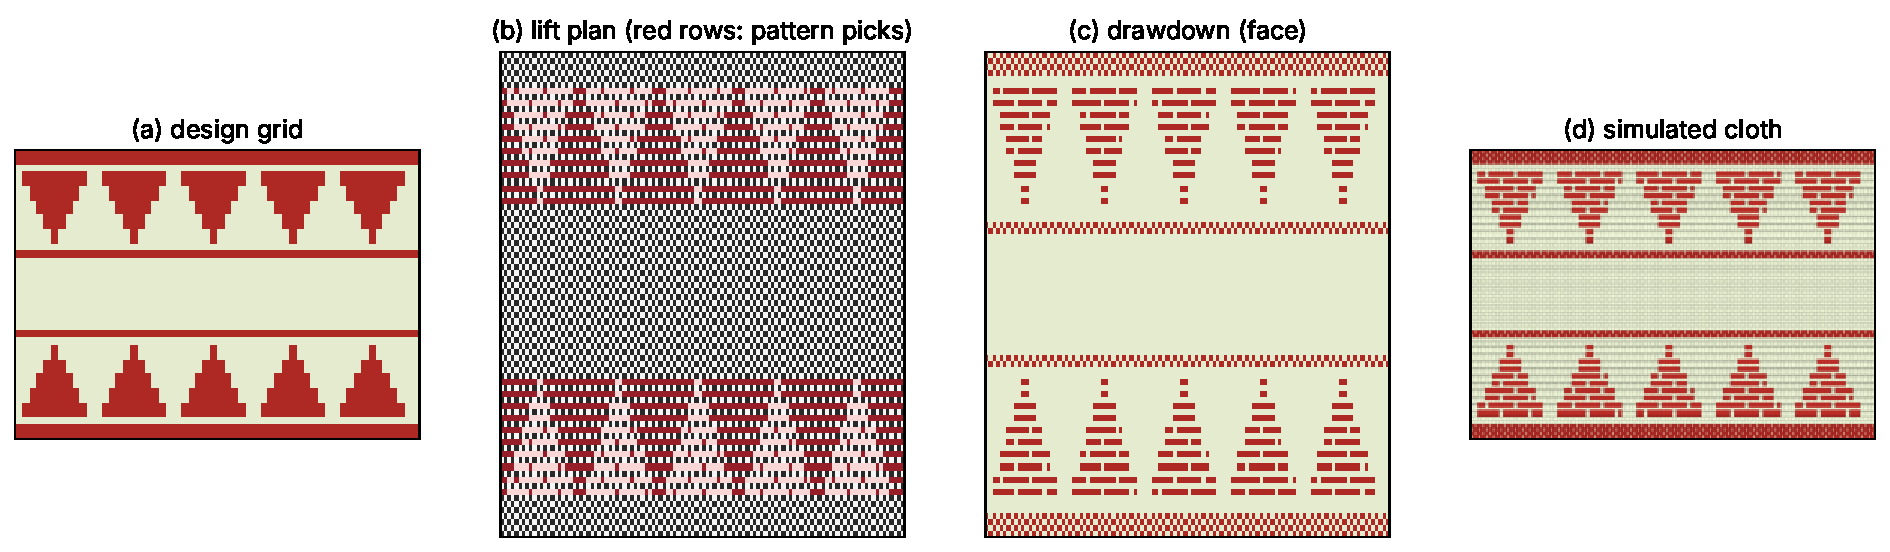
\includegraphics[width=\linewidth]{fig_compiler_pipeline}
\caption{Design to cloth: (a) design grid; (b) lift plan, pattern picks in red; (c) drawdown;
(d) simulated cloth.}
\label{fig:pipeline}
\end{figure}

\begin{figure}[t]
\centering
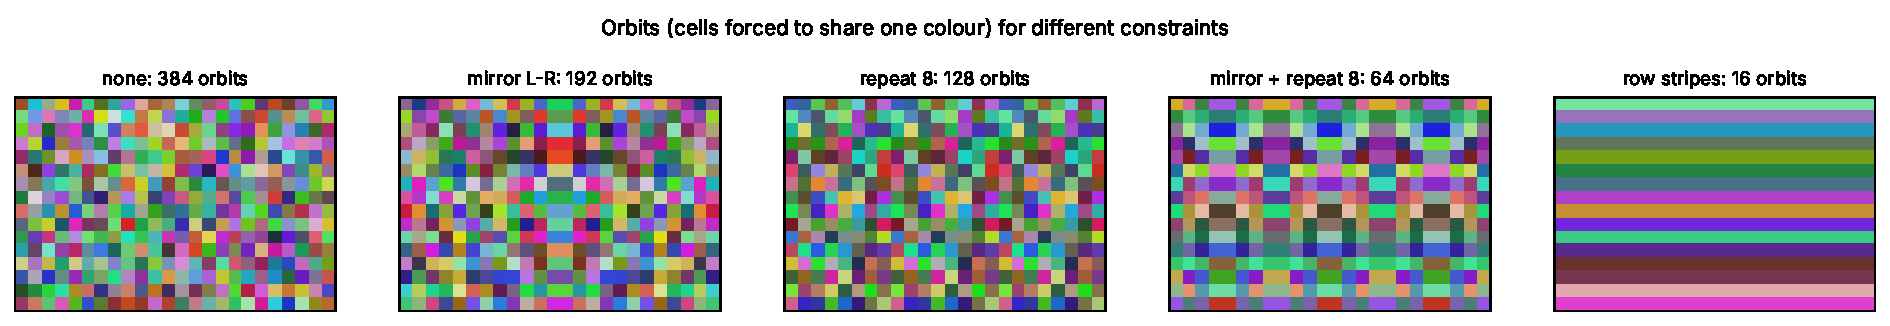
\includegraphics[width=\linewidth]{fig_orbits}
\caption{Orbits for different structural constraints; cells of one colour must agree.}
\label{fig:orbits}
\end{figure}

\begin{figure}[t]
\centering
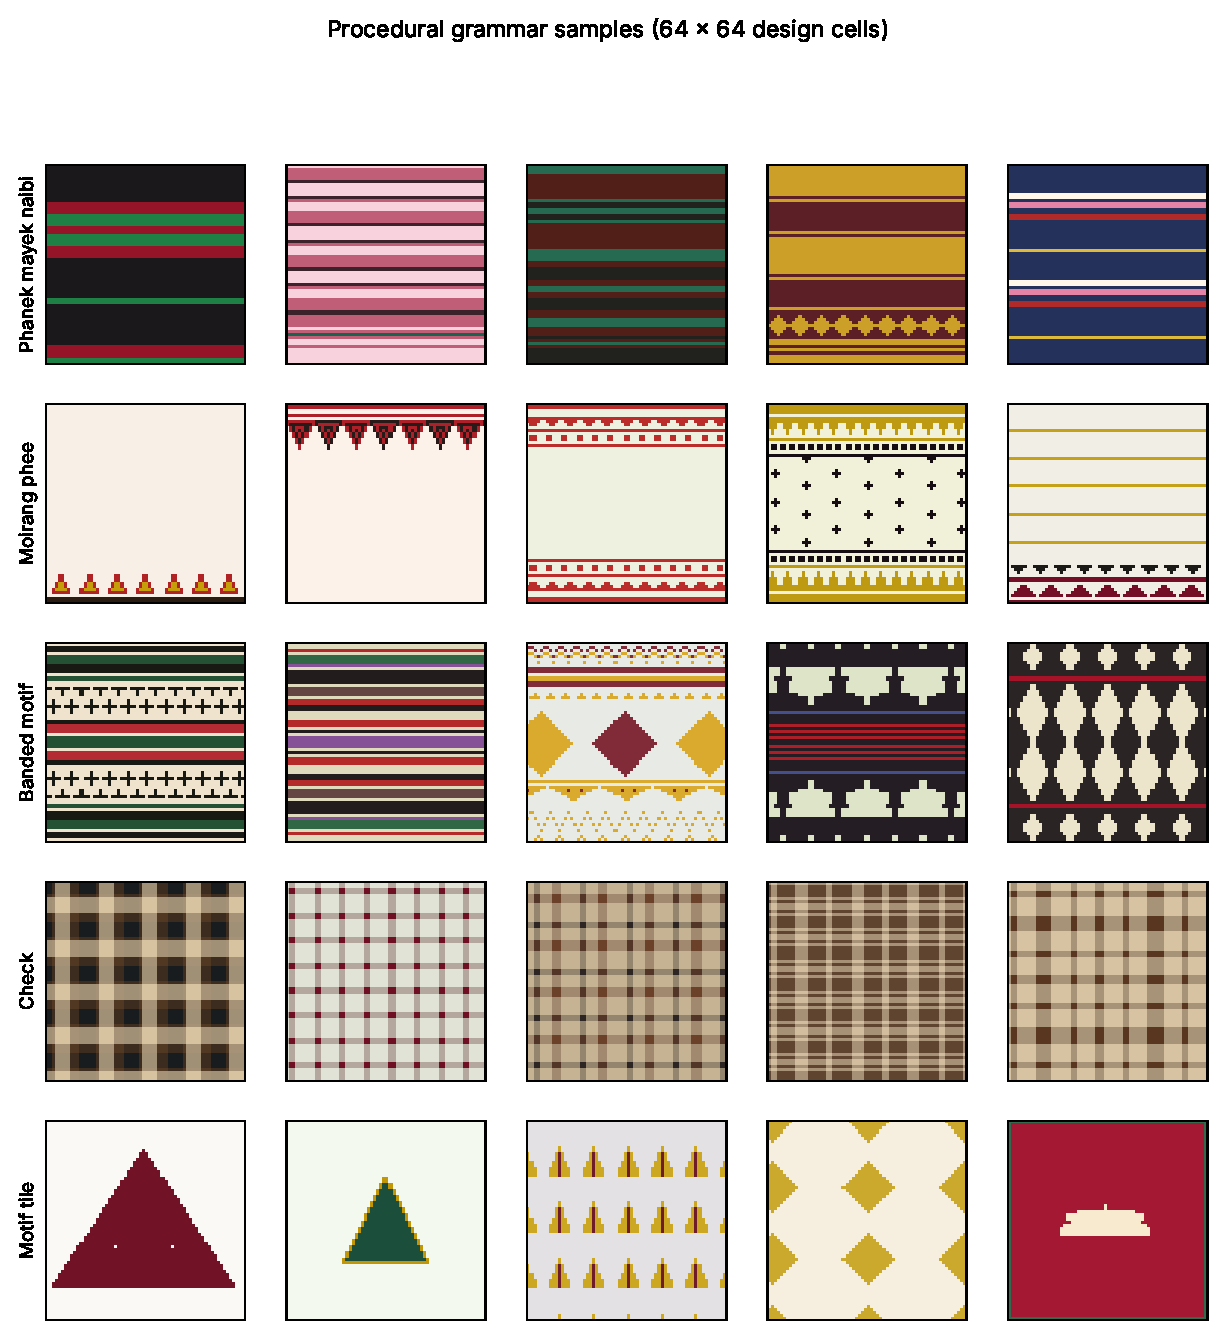
\includegraphics[width=0.85\linewidth]{fig_procedural_styles}
\caption{Samples of the procedural grammar used for pretraining.}
\label{fig:styles}
\end{figure}

%==========================================================================================
\section{Discussion and limitations}
\todo{Grid fitting on photos with strong pick structure (texton-based inference as future work);
techniques not covered (supplementary warp, embroidery, tapestry); colour modelling with yarn
catalogues; cultural and ethical considerations: consent, attribution, Geographical Indications,
benefit sharing.}

\section{Conclusion}
\todo{}

\section*{Declarations}
\noindent\textbf{Funding} \todo{} \quad
\textbf{Competing interests} \todo{} \quad
\textbf{Ethics approval and consent} \todo{} \quad
\textbf{Data availability} \todo{} \quad
\textbf{Code availability} The code is available at \todo{URL}.

\bibliographystyle{plainnat}
\bibliography{references}
\end{document}
